\chapter{Mechanising Lilac II: Proofs}
\label{chap:proofs}
\emph{Having overcome the fundamental change in the definitions, consolidate inconsistencies and instantiating Iris, we present here the 2nd aspect
of a mechanisation project: A LOT of theorem proving. We present the soundness proofs of Lilac proof rules drawing attention to 2 of them
in particular: \texttt{wp\_bind} and \texttt{wp\_unif}, due to each of them influencing the definition of the \texttt{wp}
connective (in order to validate their soundness). \texttt{wp\_bind} motivated the use of Mathlib's Probability Kernels, with kernel style definitions
and proofs. \texttt{wp\_unif} the central and most complex proof in the entire project, motivates the creation of an entire sub-library of
measure theoretic results about measurable spaces obtained through finite footprint on the Hilbert Cube.}

\fleuron{8}
% Some of the development of these proofs
% happened simultaneously with surprising progress in LLM-based auto-formalisation in Lean. We report on how these tools were used with success in simpler
% sub proofs (which are time consuming to work out but not conceptually hard), but they are not particularly good or successful, when the rich grounding of Mathlib's
% Api is not present and a library of lemmas needs to first be built in order to carry out a proof as was the case for \texttt{wp\_unif}. It is worth noting
% that as past contributor of Mathlib, Mathlib has exacting code quality standards, for the generalisability and suitable abstractions used in contributed
% code, and as seen the success of such autoformalisation is in part due to the availability of such an excellent library. The ambitions of this mechanisation
% is to form a foundation for further developments in probabilistic separation logic, such extended Lilac (with conditioning) and Bayesian Separation Logic citep{},
% so we try to maintain good abstractions and remark on the extensibility at points in the chapter.}

\Todo{Proof irrelevance for closed\_krm\_subtype also for conditioning}
\Todo{Pi-lambda theorem not suitable for BaSL}

\section{A Tour of the \texttt{wp} Connective}
\label{sec:wp}
Before we proceed with having a detailed look at any \texttt{wp} proof rule in particular, we first need to gain a strong understanding of the definition of
the \texttt{wp} connective.  We restate and motivate the definition of the \texttt{wp} connective in this
section\footnote{This is identical to the version presented before in Sec \ref{lilac}. However, in both place we have made an omission of a redundant part
of the original definition. Particularly the do-notation based equation, returns a triple rather than a tuple on both sides of the equation. The component
we have omitted, $D(\omega)$ can always be obtained by our choice in instantiation of $D\_ext$ and is hence made redundant.}:

\[
\begin{aligned}
(\mathcal{F},\mu) \vDash \mathrm{wp}(M,X\!:\!A.\,Q) &\iff \text{for all } \mathcal{P}_{\mathrm{frame}} \text{ and } \mu \text{ with } \mathcal{P}_{\mathrm{frame}}\star\mathcal{P} \sqsubseteq (\Sigma_{I^\mathbb{N}},\mu) \text{ and all } D_{\mathrm{ext}} : \mathrm{RV}\,\llbracket \Delta_{\mathrm{ext}} \rrbracket, \\
&\quad \text{there exists } X : \mathrm{RV}\,A \text{ and } \mathcal{P}' \text{ and } \mu' \text{ with } \mathcal{P}_{\mathrm{frame}}\star\mathcal{P}' \sqsubseteq (\Sigma_{I^\mathbb{N}},\mu') \text{ such that } \\
&\quad \left( \begin{array}{l} \omega \leftarrow \mu;\\ v \leftarrow M(\omega);\\ \mathrm{ret}\bigl(D_{\mathrm{ext}}(\omega),v\bigr) \end{array} \right) = \left( \begin{array}{l} \omega \leftarrow \mu';\\ \mathrm{ret}\bigl(D_{\mathrm{ext}}(\omega),X(\omega)\bigr) \end{array} \right), \\
&\quad \text{and } \mathcal{P}' \vDash Q[X]
\end{aligned}
\]

The \texttt{wp} connective is the most crucial and intricate part of the semantics of Lilac.
At the heart of the definition is the requirement that running a program with $\mathcal{P}$ as the resource, will cause a modification of the resource to $\mathcal{P'}$, such that
1) there are no unnecessary changes to $\mathcal{P}$, and 2) $\mathcal{P'}$ is able to generate the output of the program $M$.
These clauses are captured respectively, by the following splitting:
\begin{align}
\left(
\begin{array}{l}
\omega \leftarrow \mu;\\
\mathrm{ret}\bigl(D_{\mathrm{ext}}(\omega)\bigr)
\end{array}
\right)
&=
\left(
\begin{array}{l}
\omega \leftarrow \mu';\\
\mathrm{ret}\bigl(D_{\mathrm{ext}}(\omega)\bigr)
\end{array}
\right)
\qquad&
\left(
\begin{array}{l}
\omega \leftarrow \mu;\\
M(\omega)
\end{array}
\right)
&=
\left(
\begin{array}{l}
\omega \leftarrow \mu';\\
\mathrm{ret}\bigl(X(\omega)\bigr)
\end{array}
\right)
\label{eq:original}
\\[1ex]
(D_{\mathrm{ext}})_\#\mu
&=
(D_{\mathrm{ext}})_\#\mu'
\qquad&
\mu \bind M
&=
X_\#\mu'
\label{eq:simplified}
\end{align}


Firstly we see that neither measure associated with the resources, $\mathcal{P}.\mu$ or $\mathcal{P'}.\mu$ get used directly. Instead, we use $\mu$ and $\mu'$ respectively, which is any larger measure
on the Borel $\sigma$-algebra on the Hilbert cube. On the left, we see that if we choose arbitrarily some random variable $D_{ext}$ we can accommodate for the random variable to be unchanged,
with our choice of $\mu'$\footnote{We are not saying that every random variable will remain unchanged, the ordering of the quantifiers in the semantics of \texttt{wp} is crucial}.
This is in line with ``no unnecessary changes''. On the right we can see that the new measure $\mu'$ essentially encodes composition of the old resource and the program.

We will see why $D_{ext}$ is required when explaining the soundness proof for the \texttt{wp\_bind} rule (Sec \ref{sec:wp-bind}). We notice that $\mu'$ is barely constrained; it is existentially quantified and only needs
to satisfy $\mathcal{P'} \sqsubseteq (\Sigma_{I^\mathbb{N}},\mu')$. What is $\mathcal{P'}$ constrained by? The clause $\mathcal{P'} \vDash Q$. $\mathcal{P'}$ must satisfy $Q$ which having
access to $X$ will likely make assertions about it.

We have not yet mentioned $\mathcal{P}_{\mathrm{frame}}$. This aspect of the semantics is in line with what is standard in separation logic to establish the frame rule, \texttt{wp\_frame}. Fig \ref{sec:proof-rules}
lists all the \texttt{wp} of Lilac. We have proven the soundness of these rules in Lean. However, we cannot go through all of them in this report.

\begin{figure}[tb]
\centering
\begin{mathpar}
\inferrule*[right=\textsc{wp-consequence}]
  {P \vdash Q}
  {\mathrm{wp}(M,X,P) \vdash \mathrm{wp}(M,X,Q)}

\inferrule*[right=\textsc{wp-frame}]
  {X \notin F}
  {F * \mathrm{wp}(M,X,Q) \vdash \mathrm{wp}(M,X,F * Q)}

\inferrule*[right=\textsc{wp-disjunction}]
  {}
  {\mathrm{wp}(M,X,P) \lor \mathrm{wp}(M,X,Q) \vdash \mathrm{wp}(M,X,P \lor Q)}

\inferrule*[right=\textsc{wp-ret}]
  {}
  {Q[\![M]\!/X] \vdash \mathrm{wp}([\![\mathrm{ret}\;M]\!],X,Q)}

\inferrule*[right=\textsc{wp-bind}]
  {}
  {\mathrm{wp}([\![M]\!],X,\mathrm{wp}([\![N]\!],Y,Q)) \vdash \mathrm{wp}([\![X \leftarrow M;\,N]\!],Y,Q)}

\inferrule*[right=\textsc{wp-unif}]
  {}
  {(\forall\,X\!:\!\RV \mathbb{R}.\;X\sim\mathrm{Unif}[0,1]\wand Q)\vdash \mathrm{wp}([\![\mathrm{unif}\,[0,1]]\!],X\!:\!A,Q)}

\inferrule*[right=\textsc{wp-flip}]
  {}
  {(\forall\,X\!:\!\RV \mathrm{Bool}.\;X\sim\mathrm{Ber}\,p\wand Q)\vdash \mathrm{wp}([\![\mathrm{flip}\;p]\!],X\!:\!A,Q)}

\inferrule*[right=\textsc{wp-if}]
  {}
  {\mathrm{wp}([\![M]\!],X\!:\!A.\,\mathrm{wp}([\![N]\!],Y\!:\!A.\,Q(\mathrm{if}\;E\;\mathrm{then}\;X\;\mathrm{else}\;Y))) \vdash \mathrm{wp}([\![\mathrm{if}\;E\;M\;N]\!],X\!:\!A.\,Q)}

\inferrule*[right=\textsc{wp-for}]
  {}
  {I(1,e) * (\forall i\!:\!\mathbb{N}.\;\forall_{rv}\,X\!:\!A.\;\{I(i,X)\}\;M\;\{X'.\,I(i+1,X')\}) \vdash \mathrm{wp}([\![\mathrm{for}(n,e,i\,X.\,M)]\!],X\!:\!A.\,I(n+1,X))}
\end{mathpar}
\caption{\texttt{wp} proof rules of Lilac}
\label{sec:proof-rules}
\end{figure}

We conclude this section with a translation of \texttt{wp} to Lean:
\begin{leancode}
def wp (M : RV (⟪Ty.G A⟫)) (Q : RV ⟪A⟫ → LProp) : LProp :=
  fun Ω ↦
  ∀ Ω_fr : PSp, ∀ Ω_pre : ✓'(Ω_fr ⋆ Ω), ∀ μ,
    (↓Ω_pre).1 ≤ PSpace.mk' μ → ∀ {α: Type} {msα : MeasurableSpace α} (D_ext : RV α),
  ∃ X : RV ⟪A⟫, ∃ Ω' : PSp, ∃ Ω_post: ✓'(Ω_fr ⋆ Ω'), ∃ μ', (↓Ω_post).1 ≤ PSpace.mk' μ' ∧
  (toMK M ×ₖ det D_ext) ∘ₘ μ = (det X ×ₖ det D_ext) ∘ₘ μ' ∧
  (Q X).1 Ω'
\end{leancode}

We see quite a lot of new notation. Firstly, $\checkmark'$ is notation for \lean{Option.is_some : Option a → Bool}, stating for example that the independent combination \lean{Ω_fr ⋆ Ω} exists.
$\downarrow$ denotes unwrapping of the value within an \texttt{Option} when we know it is \texttt{some}. We see that the choice of random variable \texttt{D\_ext} can be to any $(\alpha, ms\alpha)$.
As suggested in Equations \ref{eq:original} and \ref{eq:simplified}, the large ``do-notation'' based equation from the informal definition of the \texttt{wp} connective can
be converted to point-free form.
In the lean code too we have a point free formulation of the equation, which essentially merges the two point free forms above. This style is adopted since it uses the
``kernel API'', Mathlib's preferred style~\citep{remy} for expressing these kinds of equations. The ``kernel API'' has vast library of lemmas, and one can imagine
how using a point free style facilitates prerequisites for applying a lemma to be more easily inferred (less parameters less things to infer), by the workhorse of type-class inference~\citep{spitters}.
Again we explain the notation. We have merged the two equations from Eq \ref{eq:simplified}, using the
$\times_k = \text{Kernel.prod} : \mathrm{Kernel}\, \alpha\, \beta \to \mathrm{Kernel}\, \alpha\, \gamma \to \mathrm{Kernel}\, \alpha\, (\beta \times \gamma)$. Remember that a kernel is defined $\mathrm{Kernel}\, \alpha\, \beta := \alpha \marrow \G \beta$.
$M$ has type isomorphic to that of a Kernel\footnote{\texttt{toMK} is a manual coercion to a kernel, which is required since denotation of Appl programs are not in general kernels, only those with Appl type \texttt{Ty.g ty}}.
\texttt{det} makes a $\RV \tysem{A}$ into a Kernel. Remember that $\RV$ is a measurable function, and a measurable function $f: \alpha \marrow \beta$ can be converted
to a kernel by lifting the output into the corresponding Dirac measure: 
$\lambda x \mapsto \mathrm{dirac}\, (f\, x) : \mathrm{Kernel}\, \alpha\, \beta$. Let us expand our diagrammatic representation to include both \texttt{det} and $\times_k$.
The latter, doesn't have any special shape associated with it and is just a splitting of wires. The former we denote with an oval inside the kernel symbol (which is the triangle, see Sec \ref{sec:appl}).
We present in Fig \ref{fig:wp-calc} the equation in the definition of \texttt{wp} that we have just discussed.
We modify our notation to be vertical instead of horizontal in preparation for writing the much larger equational reasoning arguments we will be seeing in Sec \ref{sec:wp-meas}.

\begin{figure}[tb]
    \centering
    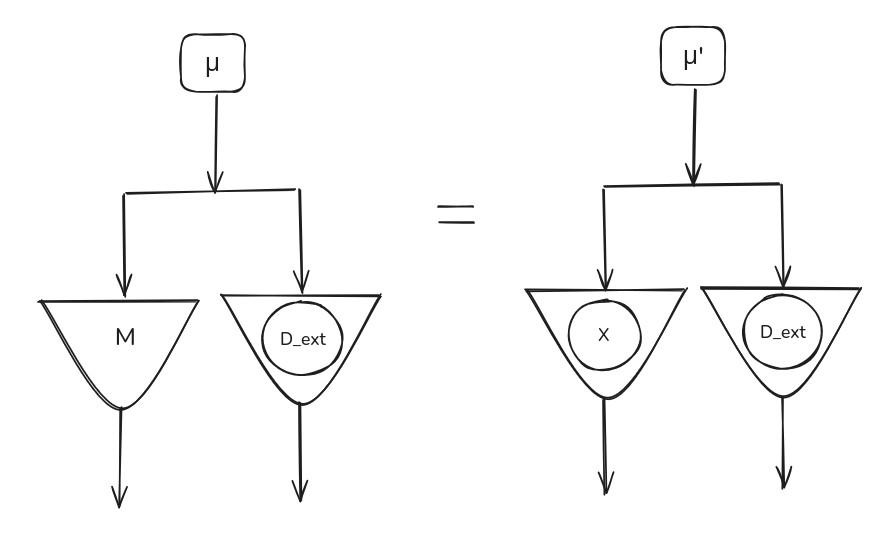
\includegraphics[width=0.65\linewidth]{proofs/wp-calc.png}
    \caption{Equational reasoning in definition of \texttt{wp}}
    \label{fig:wp-calc}
\end{figure}

\section{wp\_bind}
\label{sec:wp-bind}
This is our first presentation of the soundness of a \texttt{wp} proof rule. We will focus on getting the intuition
across to the reader, without getting weighed down by the technicalities of the Lean code. \texttt{wp\_bind} is chosen since it prominently features a different style of proof
that is significant in many of the soundness proofs of \texttt{wp} rules. Specifically, it employs equational reasoning on kernels, and Mathlib's kernel ``API'', of lemmas
allows us to stay at the level of abstraction of kernels without going down to the integrals in this proof. This is as opposed to some of the other proofs, prominently \texttt{wp\_unif}
and \texttt{wp\_flip}, which are dominated by measure theoretic proof obligations. We can understand the former as being more familiar to the computer scientist and the latter
 falling more into the mathematician's plate. We employ
the diagrammatic notation again, for a remarkably easy to understand proof of \texttt{wp\_bind}, translated into this point-free style from the original proof in \citep{lilac}.

Recall that \texttt{wp\_bind} is defined:
\[
\inferrule*[right=\qquad\textsc{wp-bind}]{}{{\color{ForestGreen} \mathrm{wp}(\sem{M},X,{\color{RoyalBlue}\mathrm{wp}(\sem{N},Y,Q)})} \vdash \mathrm{wp}(\sem{X \leftarrow M;\,N},Y,Q)}
\]
where we have colour-coded the premise with the \textcolor{ForestGreen}{outer \texttt{wp}}, and \textcolor{RoyalBlue}{inner \texttt{wp}} each yielding an equation which we will use in establishing the goal.
Recalling Sec \ref{sec:wp} in a nutshell, given a $\mu$ and program $M$, a \texttt{wp} gives back a $\mu'$ and random variable $X$ (where the $\mu$ and $\mu'$ are each associated with the old and new resource, $\mathcal{P}$ and $\mathcal{P'}$
respectively). This corresponds to the Lean code:

\begin{leancode}
theorem wp_bind (Q : RV ⟪B⟫ → LProp) (D : RV (TProd (⟪·⟫) rs))
    (M : Term rs A.G) (N : Term (A::rs) B.G)
    : wp (M.den ∘ᵣ D) (fun X ↦ (wp (N.den ∘ᵣ (X ;; D)) Q))
      ⊢ wp ((M.bind N).den ∘ᵣ D) Q := by
\end{leancode}

Our goal is to prove:

\begin{figure}[h]
    \centering
    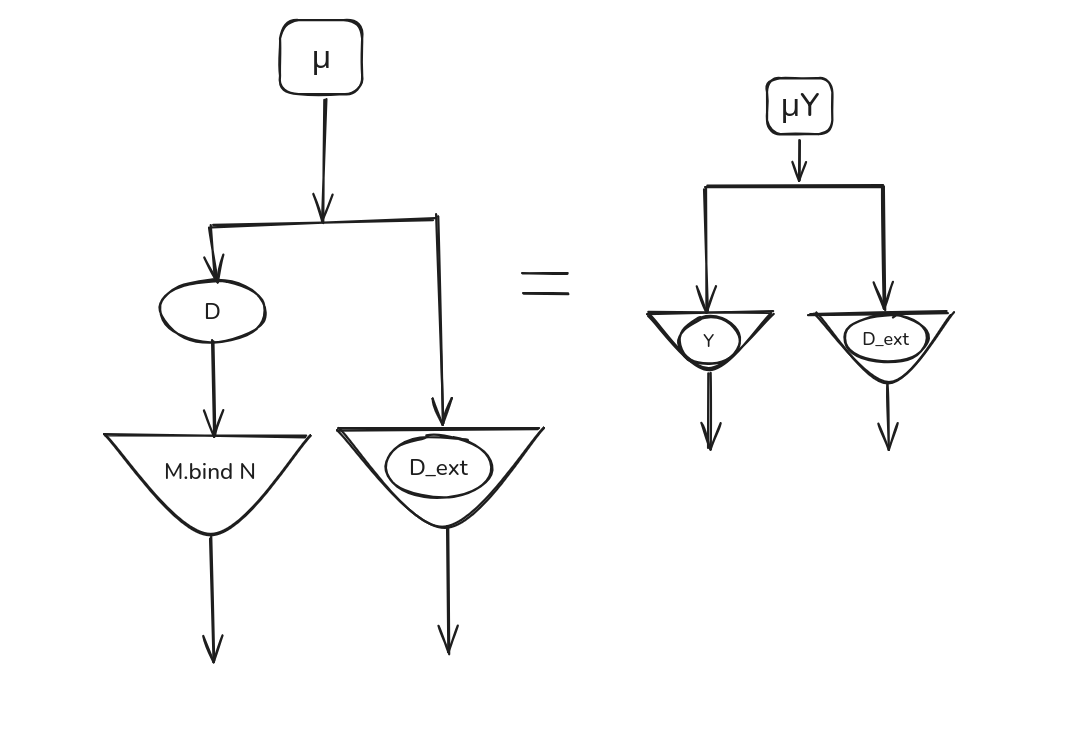
\includegraphics[width=0.65\linewidth]{proofs/bind-goal.png}
\end{figure}

We first note that we need to construct both a $\mu Y$ (a more sensible name than the usual $\mu'$) and $Y$ to satisfy the proof obligation. We notice some new notation, an oval outside a triangle?. This represents a measurable function, in our case $D$, in a random variable context. $D$ is implicit in the informal presentation but is explicit
in the Lean code. We bring clarity through the types denoting, noting that $\circ_r$ is just straightforward function composition. In Lean this composition operation is \texttt{Kernel.comap}.

\begin{align*}
\mathrm{(M.bind N).den} &: \mathrm{Kernel}\, (\mathrm{TProd}\, \tysem{\cdot}\, \mathrm{rs})\, \tysem{B} \\
\mathrm{(M.bind N).den} \circ_r D &: \mathrm{Kernel}\, I^\mathbb{N}\, \tysem{B}
\end{align*}

Continuing with the proof, we feed $\mu$ into the \textcolor{ForestGreen}{outer \texttt{wp}}, to obtain a $\mu X$ and $X$ such this equation holds:

\begin{figure}[h]
    \centering
    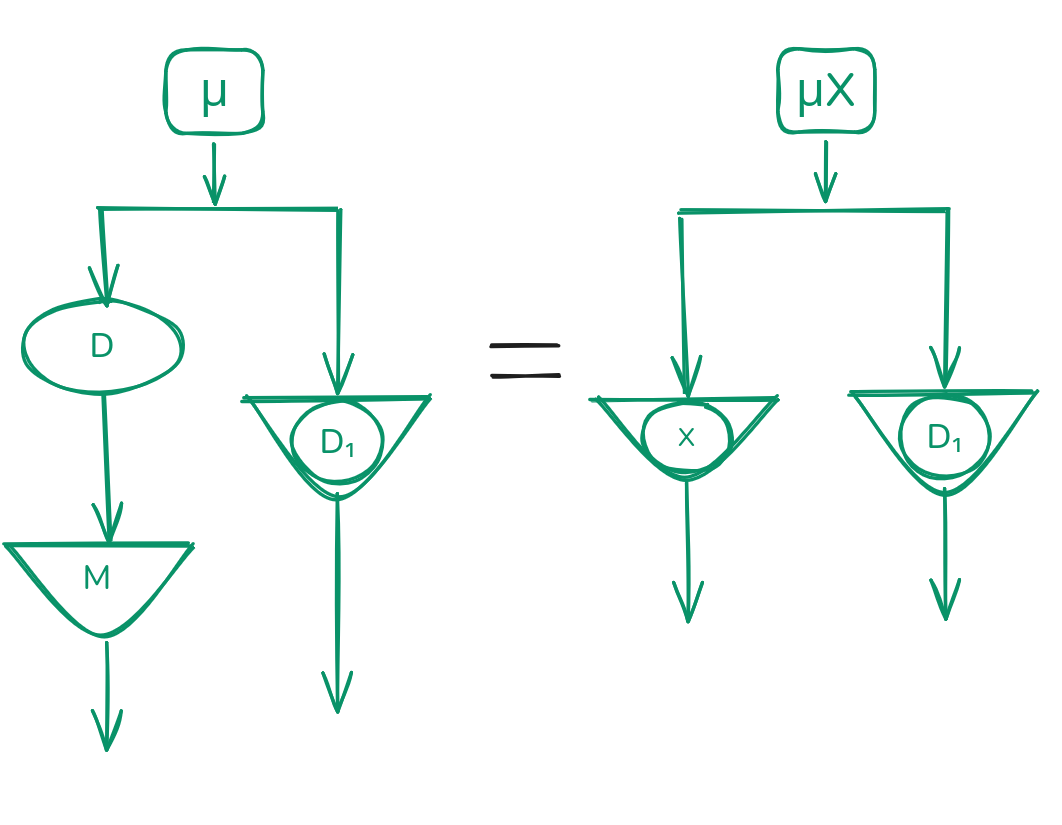
\includegraphics[width=0.5\linewidth]{proofs/bind-outer.png}
\end{figure}

Notice that since \texttt{D\_ext} is universally quantified for \texttt{wp} \texttt{LProp}, we rename to $D_1$ here to avoid name clashes. The above result can be used with any $D_1$ instantiation.

From the \textcolor{ForestGreen}{outer \texttt{wp}} we will obtain that the resource associated with $\mu X$, satisfies the \textcolor{RoyalBlue}{inner \texttt{wp}}. So feeding $\mu X$ to the \textcolor{RoyalBlue}{inner \texttt{wp}},
further provides $\mu Y$ and $Y$ such that this equation holds:

\begin{figure}[h]
    \centering
    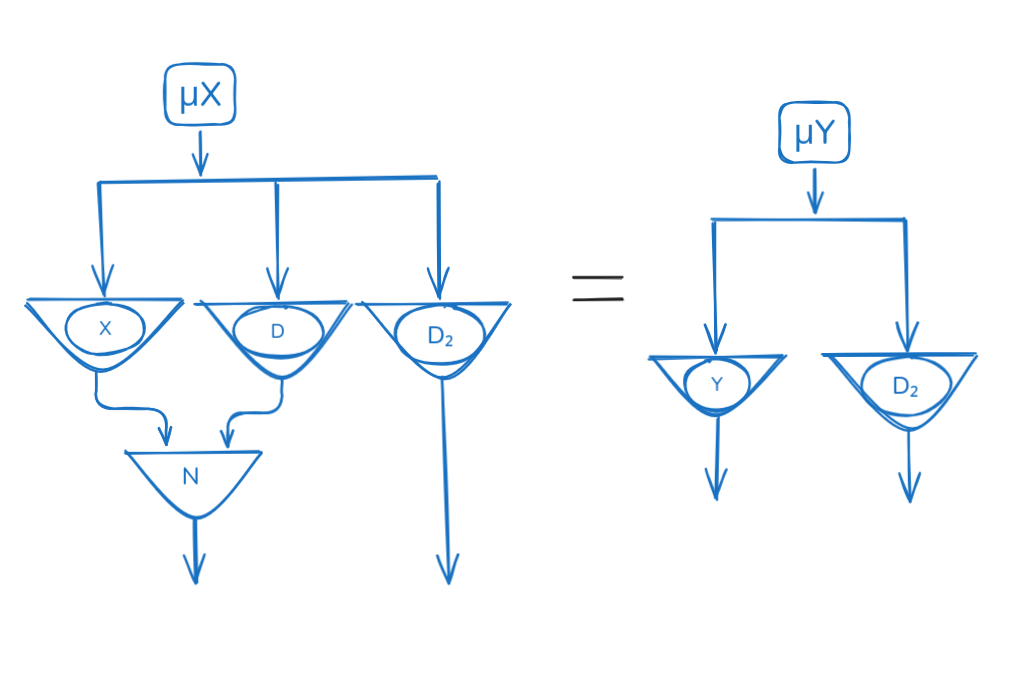
\includegraphics[width=0.65\linewidth]{proofs/bind-inner.png}
\end{figure}

Notice that it seems like $N$ is receiving two inputs but that is just the usual random variable context, extending with the $X$ obtained from running $M$. We put everything together 
to achieve the goal (given above in black) in Fig \ref{fig:bind-proof}.

Notice that we refer to application of the premises in our proof using their respective colours. When applying \textcolor{ForestGreen}{outer \texttt{wp}}, we instantiate $D_1 =$ \texttt{D;;D\_ext}, and
when applying \textcolor{RoyalBlue}{inner \texttt{wp}} we instantiate $D_1 =$ \texttt{D\_ext}.

\begin{figure}[bp]
    \centering
    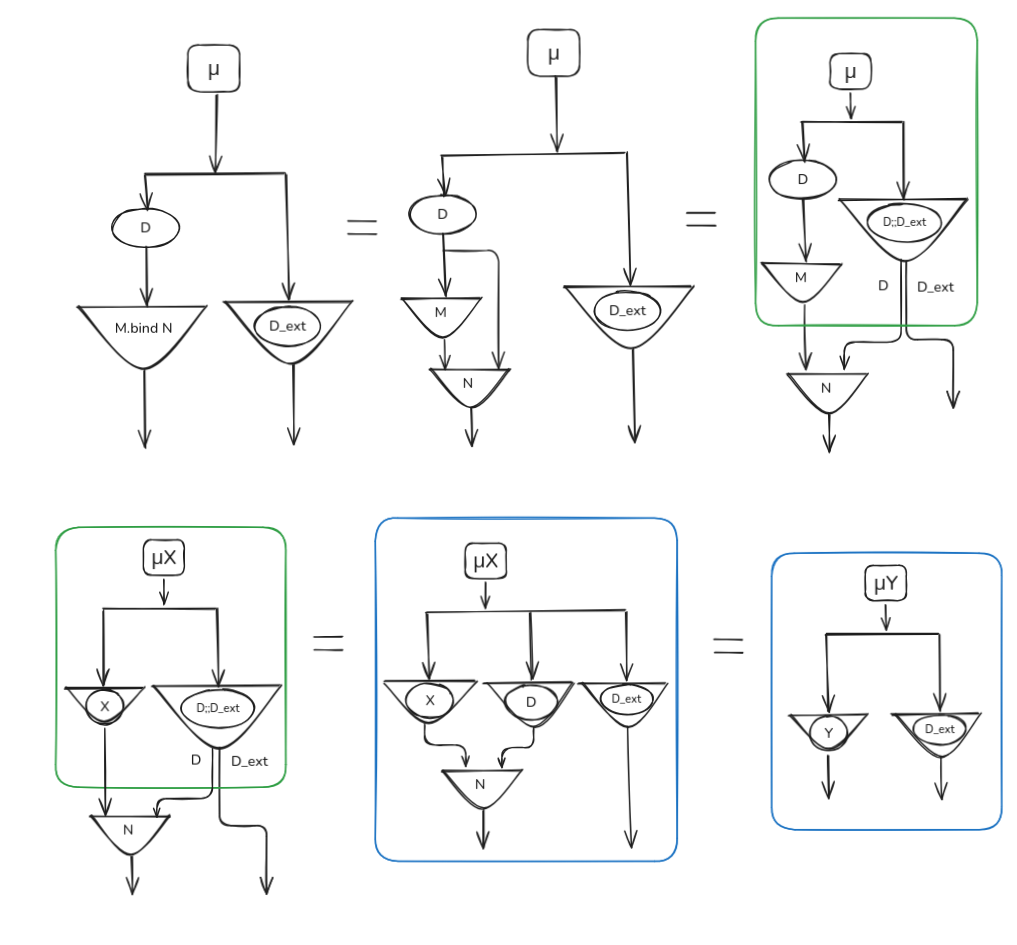
\includegraphics[width=1.0\linewidth]{proofs/bind-proof.png}
    \caption{A proof of soundness of the \texttt{wp\_bind} rule in our custom diagrammatic notation for (point-free) equational reasoning}
    \label{fig:bind-proof}
\end{figure}

We conclude with some commentary of how the connection between \texttt{wp\_bind} with \texttt{wp\_unif} and \texttt{wp\_flip} affected the process of mechanisation in practice.
Note that we actually prove \texttt{wp\_meas}, a generalisation of \texttt{wp\_unif} and \texttt{wp\_flip}
that we will refer to from here. It is explained immediately in the next section \ref{sec:ff}.
Unlike \texttt{wp\_meas}, \texttt{wp\_bind} is a standard rule
in any weakest precondition based logic. However, it is deeply intertwined with the semantics of \texttt{wp}, adding the extra bookkeeping of
\texttt{D\_ext} to the definition of the \texttt{wp} connective. Indeed \texttt{wp\_unif} and \texttt{wp\_bind} can be understood as reinforcing each other's
difficulty! During the mechnaisation we approached these two proofs in an interleaved fashion. We first proved soundness of \texttt{wp\_unif}, whilst redefining \texttt{wp} to remove all occurrences of \texttt{D\_ext}.
Reducing the complexity of \texttt{wp} brought the soundness proof of \texttt{wp\_unif} within approachable distance, so it was deemed necessary, even if we needed to
add \texttt{D\_ext} back in later and rework the proof. Then on attempting to prove \texttt{wp\_bind} and realising why it is unprovable without \texttt{D\_ext}, \texttt{D\_ext}
was added back in. Then \texttt{wp\_unif}'s proof obligation got a little harder but most of the measure theory lemmas where either already there, could
be generalised or adapted for the new proof obligations. \texttt{wp\_unif} and \texttt{\wp} both proofs completed.

\section{Finite Footprints}
\label{sec:ff}
When it comes to the proof rules of Lilac, the probability-specific reasoning that can occur in the logic is predominantly present in two rules \texttt{wp\_unif} and
\texttt{wp\_flip}, which reason about two syntactic constructs from Appl, \texttt{unif01} (uniform distribution on unit interval) and \texttt{flip}
(bernoulli distribution) respectively. There is nothing special about these two distributions, and we can indeed have a general rule \texttt{wp\_meas}, parametric
over any distribution. For this suppose we define a new Appl term, we also introduce a construct for defining a general distribution, like so:

\[
\tag{\textsc{wp-meas}}
(\forall\, X : \RV A.\; X \sim \mu \wand Q)
\;\vdash\;
\mathrm{wp} (\lambda\ \_ \mapsto \mu) ( \lambda X\!:\!A.\mapsto Q)
\]

where $\mu$ is an arbitrary probability measure. We are specifying a denotation directly instead of taking the denotation of some concrete program.
Note that $(\lambda\ \_ \mapsto \mu) : A \marrow \mathcal{G} B$ which is correctly typed as a denotation of a program
(in other words it is a kernel).

The soundness of \texttt{wp\_meas} is the general theorem that we prove in lean and instantiate to \texttt{wp\_unif} and \texttt{wp\_flip}. The choice of the Hilbert Cube
with finite footprint as a probability space was made to validate \texttt{wp\_meas}. In order to prove the soundness of this result, we first had to establish a
substantial body of fundamental results in Lean about Hilbert cubes with finite footprint, to express transformations which are so intuitive that they do
not even get mentioned in proof in Lilac's appendix, but nevertheless, took weeks of effort. The reason for this difficulty boils down to the fact that Finite footprints
were invented for validating these proof rules, and isn't of general mathematical interest to be supported by Mathlib.

\textbf{Definition B.5 \citep[Appendix B]{lilac}} A sub-$\sigma$-algebra $\mathcal{F}$ of $\Sigma_{I^\mathbb{N}}$ has finite footprint if there is some n such that every $F \in \mathcal{F}$
is of the form $F' \times [0,1]^\mathbb{N}$ for some $F' \subseteq [0,1]^n$.

The intuition behind this definition goes back to the slogan ``measurability is ownership''. Finite footprint restricts the set of measurable functions from the
Hilbert cube (thereby restricting ownership over random variables). We have adopted the below equivalent definition which makes the intuition explicit, at the cost of
introducing a few more concepts (the change motivated making the proofs clearer and succinct). The following snippets are from \repo{Std}.

\begin{leancode}
/-- The σ-algebra is only "interesting" in the first `n` coordinates for
some finite `n`.  In the rest of the coordinates, its the `univ` set. -/
def FiniteFootprint (n : ℕ) (ms : MeasurableSpace (ℕ → I)) : Prop :=
  ∃ ms' : MeasurableSpace (Fin n → I), ms = unSplitBi (ms' ×ₘ (⊥ : ℕ → I))
\end{leancode}

First let's look at the types involved $\mathbb{N} \to I$ is exactly the Hilbert cube, while $\mathrm{Fin}\ n \to I$ ($I^n$) is a finite portion of it.
There exists an isomorphism $(\mathrm{Fin}\ n \to I) \times (\mathbb{N} \to I) \simeq \mathbb{N} \to I$, which just says that we can split something infinite to a
finite and infinite part.

We define finite footprint based on this isomorphism, defined in Lean as \texttt{splitBi}:

\begin{leancode}
noncomputable def splitBi (n : ℕ) : (ℕ → I) ≃ᵐ (Fin n → I) × (ℕ → I) :=
  (MeasurableEquiv.piCongrLeft (fun _ => I) (finSumNatEquiv n)).symm.trans
  (MeasurableEquiv.sumPiEquivProdPi (fun _ => I))
\end{leancode}

We focus on the type of splitBi; $\simeq^m$ is notation in mathlib for measurable equivalence, lifting the isomorphism just presented above for the types,
to measurable spaces, i.e. there are measurable functions going back and forth, with composition in each way giving the left or right identity functions.
(The body of the definition is using results from Mathlib, and is just constructing such an isomorphism)

\texttt{splitBi} is the natural notion of isomorphism between measurable spaces that we chose for defining finite footprints, finally here is unsplitBi,
which is applying the splitBi backwards, from the split measurable space to the ``unsplit'' space by taking the pullback $\sigma$-algebra, which is called \texttt{comap}
in Lean.

\begin{leancode}
abbrev unSplitBi {n : ℕ} (ms : MeasurableSpace ((Fin n → I) × (ℕ → I)))
    : MeasurableSpace (ℕ → I) := ms.comap (splitBi n)
\end{leancode}

Now returning to the definition \texttt{FiniteFootprint}, we see that we are choosing some arbitrary measurable space on the finite part, and the
measurable space $\bot = \{\phi, I^\mathbb{N}\}$ on the infinite part. This smallest/trivial measurable space on the infinite part of the hilbert
cube, makes that part effectively meaningless. A random variable mapping from a finite footprint hilbert cube (thought of as an infinite list),
would be forced to ignore all indices greater than n (
from the infinite part). We offer a way to visualise a measurable space over the hilbert cube in \ref{fig:hc}.

\begin{figure}[tb]
  \centering

% \TwoPhasePartitionGraph{1234}{15}{8}{10}
% \TwoPhasePartitionGraph{42}{15}{8}{10}
% \TwoPhasePartitionGraph{43}{15}{8}{10}
% \TwoPhasePartitionGraph{44}{15}{8}{10}
\caption{A suggestion for visualising a Finite footprint measurable space over a hilbert cube. The entire diagram is a single measurable space. Each strip
makes up the measurable sets (or events) in the space. Each line in represents an infinite tuple of reals in the unit interval, connecting dots which single reals,
on a vertical number line. Note that beyond the finite footprint, the lines get dense. In a fully faithful diagram, that part would be entirely filled in.}
\label{fig:hc}
\end{figure}


Let's take a quick example, to see why indices after n must be ignored. Take $X : I^\mathbb{N} \to Bool$, and a finite footprint measurable space over the domain
and the powerset measurable space over the codomain ($\{\phi, \{false\}, \{true\}, \{false, true\}\}$).

Let's say we know $X(0.1, 0.1, 0.1, \ldots) = false$. 
Then what is the pre-image of the measurable set {false} constrained to be, to remain measurable? The smallest possible answer is $X^{-1} (\{false\}) = (0.1, 0.1, a_0, a_1, a_2, \ldots)$
for arbitrary $a_i \in I$. Referring to Fig \ref{fig:hc}, this is the same as saying that the region past n, is dense. Hopefully, this convinces the reader
of the key fact that a random variable (which is a measurable function) from a finite footprint Hilbert cube, must ignore all the dimensions beyond n, in
other words Finite footprint hilbert cube (FFHC) can't own every random variable and are restricted in some way. In particular, we are always able to easily construct
random variables that a FFHC does not own simply by having some $Y$ consider the values of dimensions greater than n.

The above FFHC property of measurability interpretable as ownership, only used the fact that FFHC can be decomposed into a product. So it is just
a property of product measurable spaces. The key property of a lilac resource $\mathcal{P} = (\Sigma_{I^\mathbb{N}}, \mathcal{F}, \mu)$ (FFHC along with a probability measure) is one can create
a new $\mathcal{P'} = (\Sigma_{I^\mathbb{N}}, \mathcal{F'}, \mu')$ by ``adding a random variable $Y$ to $\mathcal{P}$''.
Let's make that intuition precise.

\begin{enumerate}
\item For all random variables $X : (I^\mathbb{N}, \mathcal{F}) \marrow A$ (we explicitly state the measurable space of
the domain), which we refer to as random variables owned by $\mathcal{P}$, $X$ must also be measurable w.r.t. $\mathcal{F'}$.
\item Say we have a probability
measure $\nu$ in the space $B : \texttt{Meas}$. We are able to construct $\mathcal{P'}$ such that with a suitable choice of $Y : (I^\mathbb{N}, \mathcal{F'}) \marrow A$,
$Y_\#\mu' = \nu$!
\end{enumerate}

Let's show concretely how to construct both $\mathcal{P'}$ and $Y : I^\mathbb{N} \marrow \mathbb{R}$, taking $\mathbb{R}$ as the co-domain and
the target distribution $\nu=\mathrm{Unif}[0,1]$ to be the uniform distribution on the unit interval,
in this example. Let $\mathcal{P}$ have finite footprint n. The idea is to first construct a $\mathcal{P}_n = (I^\mathbb{N}, \mathcal{F}_n, \mu_n)$, 
where we can define $Y$ as a projection  $Y := (\omega : \mathbb{N} \to I) \mapsto \omega n$ to obtain the target distribution $Y_\#\mu_n = \nu$.
$\mathcal{P}_n$ satisfies condition (2) above while the original $\mathcal{P}$ of course satisfies (1), but neither satisfies both. We claim that taking the
independent combination $\mathcal{P'} := \mathcal{P} \star \mathcal{P}_n$ will satisfy both conditions. Deferring the justification of this claim to
the next section \ref{sec:wp-meas}, we provide the construction of $\mathcal{P'}$ here.

The Hilbert cube can be decomposed into product measurable spaces
at arbitrary indices n. The construction of $\mathcal{P}_n = (I^\mathbb{N}, \mathcal{F}_n, \mu_n)$, is defined using a decomposition of the hilbert cube
into 3 pieces: before n, at n and after n.

$(I^\mathbb{N}, \mathcal{F}_n) \simeq^m (I^n, \bot) \times_m (I, \Sigma_I) \times_m (I^\mathbb{N}, \bot)$

We also need to define $\mu_n$. On the trivial measurable space $\bot = (I^x, \{\phi, I^x\})$ measurable space there is only one possible probability measure defined as $\mu_\bot := \{\phi \mapsto 0, \mathrm{univ} \mapsto 1\}$.
$\mu_n := \mu_\bot \otimes \lambda_I \otimes \mu_\bot$. Where $\lambda_I$ is the Lebesgue measure on $I$ and $\otimes$ is the product of measures (see Sec \ref{sec:measure-theory}).

Note that $\lambda_I$ expanded into a measure on $\mathbb{R}$ (mapping all new elements from its domain to 0), is precisely $\nu=\mathrm{Unif}[0,1]$. So if $Y$ is a map from
$\mathcal{P}_n$, we get $Y_\#\mu_n = \mathrm{Unif[0,1]}$ as required. We wish that if we take the independent combination $\mathcal{P'} := \mathcal{P} \star \mathcal{P}_n$,
then we will also have $Y_\#\mu' = \mathrm{Unif[0,1]}$

We are now in a position to state a 3rd slogan: ``Hilbert Cubes with Finite Footprint are infinite random number generators''. Given some resource $\mathcal{P}$ representing
the state of a program, we are always able to modify this state to some $\mathcal{P'}$ which supports one more random variable $Y$ of our choice. Each of these $Y$s are
just straightforward projections of some dimension n, i.e. measure on each dimension is the source of randomness. And we can repeat this process arbitrarily, because
of the finite footprint condition, obtaining a resource
which simultaneously supports an arbitrary number of random variables $Y_i$.

We end this section with the definition of a finite footprint for a measurable function:

\textbf{Definition B.6 \citep[Appendix B]{lilac}} A random variable $X : (I^\mathbb{N}, \Sigma_{I^\mathbb{N}}) \to (A, \Sigma_A)$ has finite footprint if the pullback $\sigma$-algebra $\{X^{-1}(E) \mid E \in \Sigma_A\}$ has finite footprint.

The need for this definition is a technical detail: sometimes we will not always have access to a measurable space with finite footprint to define a measurable map from. Even when a measurable function
is from the Borel $\sigma$-algebra on the Hilbert cube, this definition allows us to only consider those measurable maps, which still behave as if they were mapping from some $\sigma$-algebra
with a finite footprint. We will see an example of this in use in Sec \ref{sec:wp-bind}.

\section{wp\_meas}
\label{sec:wp-meas}

In Sec \ref{sec:ff} on Finite Footprints we gave most of the intuition for the proof of the rule \texttt{wp\_meas} followed by defining precisely the semantics of \texttt{wp}, which appears in
\texttt{wp\_meas}, in Sec \ref{sec:wp}. Now we can discuss the proof of soundness of \texttt{wp\_meas}, elaborating on Sec \ref{sec:ff} and showing parts of the Lean mechanisation.

In our presentation of transformations on the Hilbert cube, we are being quite verbose with stating the isomorphisms (measurable equivalence), by ``splitting'' and ``unsplitting'' the Hilbert cube. In the
informal proof this isomorphism is not mentioned, and it is natural to fluidly move in between the two representations, not even noticing that there must in
fact be two different representations in a type theory (since the types $I^\mathbb{N}$ and $I^n \times I^\mathbb{N}$ are not equal). At the base there is a measurable equivalence on measurable spaces,
and on top of that there is also an isomorphism of measures over
each representation. In Sec \ref{sec:ff} we had brushed over this as is done in the informal proof, appealing to intuition. However, this isomorphism between the measures is not covered by
Mathlib, so as part of this project we have had to develop some deep measure-theoretic results which are not directly related to finite footprints.
This is one of the factors which makes the proof of \texttt{wp\_meas} the hardest in the entire development, and ended up taking weeks instead of days.
We had hoped to talk here about the specific gaps in Mathlib's infrastructure, presenting it in full detail. However, this introduces a lot of notation
and details of the reasoning steps in the proofs, to reach a rather technical point in the grand scheme of the entire formalisation. So instead, we will
not present the details of 



 we talk specifically about the
measure-theoretic result which lets us make some remarks on some incompatibilities of Mathlib (or mainstream mathematics) with our requirements which has plagued most proofs across the development to some extent.

\[
\tag{\textsc{wp-meas}}
(\forall\, X : \RV A.\; X \sim \mu \wand Q)
\;\vdash\;
\mathrm{wp} (\lambda\ \_ \mapsto \mu) ( \lambda X\!:\!A.\mapsto Q)
\]

We want to prove a \texttt{wp} statement.

Taking some $\mathcal{P}$ for which the premise holds, our goal is to 
validate $\mathcal{P} \vDash \mathrm{wp} (\lambda\ \_ \mapsto \mu) ( \lambda X\!:\!A.\mapsto Q)$.
To validate a \texttt{wp} connective, one of the things we require is to construct a new $\mathcal{P'}$ which owns a random variable $X$ whose distribution
is $\mu$. Mathematically stated, given $\mathcal{P'} = (\Sigma_{I^\mathbb{N}}, \mathcal{F}, \mu')$, 

In order to see what is required to achieve this rule we first need to remember
the semantics of the $\wand$. 
$X \sim \mu \wand Q$ holds for some $\mathcal{P}$ if we have $\mathcal{R} \vDash X \sim \mu$, and $\mathcal{R} \star \mathcal{P}$ exists then
$\mathcal{R} \star \mathcal{P} \vDash Q$. If the premise above holds, then 

We need to 

$ \mathcal{R} \vDash P \wand Q$ if there is some $\mathcal{P} \vDash P$
\Todo{How do I talk about anything hard without getting bogged down with explaining easy stuff. I think I should just give up on re-explaining
proofs. It makes no sense there's already a paper, and I've formalized it so why another version :(}

We begin with this equality at the heart of the proof.
\begin{leancode}
lemma commute_with_add_dim {N : ℕ} (N_ms : MeasurableSpace (Fin N → I))
    : unSplitTri ((N_nil N) ×ₘ I_borel ×ₘ Inf_nil) ⊔ unSplitBi (N_ms ×ₘ Inf_nil)
      = unSplitTri (N_ms ×ₘ I_borel ×ₘ Inf_nil) := by ...
\end{leancode}
Recalling the development from Sec \ref{sec:ff} this proof is essentially $\mathcal{P}_n \star \mathcal{P} = \mathcal{P'}$ (in that order in the Lean code) but only showing the
equality for the underlying measurable space, forgetting the measure. For example, if \texttt{.ms} denotes the underlying measurable space then
$\mathcal{P}.\mathrm{ms} = \mathrm{unSplitTri}((\mathrm{N\_nil}\; N) \times_m \mathrm{I\_borel} \times_m \mathrm{Inf\_nil}) = (I^\mathbb{N}, \mathcal{F}_n) \simeq^m (I^n, \bot) \times_m (I, \Sigma_I) \times_m (I^\mathbb{N}, \bot)$.
Note that the independent combination $\star$, cast down to measurable spaces, is the sum of the two measurable spaces: the smallest $\sigma$-algebra generated from the union
of the two spaces. This is also \texttt{join} $\sqcup$ (measurable spaces form a lattice), which is what we see in Lean.

There was a slight omission in the above presentation, regarding the presence of $\mathcal{P}_{\mathrm{frame}}$

We want this result to extend to the relevant measures on these spaces clearly. This is the contents of the file \repo{ProofRules/MeasureProduct}. There we
prove lemmas to establish this result as stated. However ideally we could generalise this result much further to just be about an isomorphism between
measures when there is a measurable equivalence between two spaces, which are some combination of products and sums. Our current proofs are tied
to the definitions of finite footprint and the specifics of PSLs like Lilac, but it would be much nicer, to add these general theorems about how measures are
isomorphic over different measurable equivalences over spaces constructed with sums and products in Mathlib. This is important future work, to ensure
the readability and extensibility to newer logics for the Lean codebase.

\subsection{Use of Aristotle in this proof}
Here we outline our usage of \href{https://aristotle.harmonic.fun/dashboard}{Aristotle}, a public free Generative model, which is intended specifically for
writing Lean code. There has been astonishing progress in the successfulness of AI in writing valid Lean proofs, within the duration of the project.
We tried Claude, at the end of 2025 to try to fill in some proof holes, and it was not particularly useful and abandoned, along with all AI generated code.
However, when attempting to use these tools again in within the previous month or two (specifically we have tried only Aristotle) these tools are now consistently
at the level of automating the proofs of time-consuming but trivial helper lemmas of a few lines each. Specifically by ``helper lemma'' we actually refer
to \texttt{have := ...}, statements peppered throughout all the proofs. This being the first mechanisation project of this scale in my experience, I
had learned at some point that it was a terrible idea to fill every hole in every proof, and always keep the codebase in a coherent state. It is instead a
much better approach to repeatedly quash the biggest uncertainties of the shape of the mechanisation: for example the interface between the language and logic,
the interface between logic and Iris, whether verification of an open program (containing a free variable) is possible, the soundness proofs
of probability specific proof rules, and their usage. It was important to trust intuition and develop the project as a patchwork of proofs that slowly come together,
to get the most accurate idea of how much time each part would take and avoid wasted effort on a proof, that might need to be reworked. The approach naturally
left behind a lot of trivial holes, which we're exactly the right size for having Aristotle fill, since morally, there was only 1 right answer.

The biggest issue with using Aristotle with larger or difficult tasks, it may pursue terrible ideas, and give a very wrong impression of the difficulty and
the best approach of proving a difficult theorem, especially when there are ambiguities and choices to be made. The proof of \texttt{wp\_meas} is where
Aristotle was inadvertently used the most, hence we include this reflection here. Firstly, as mentioned before the pure measure theoretic results,
where so intuitive that they were stated as ``by definition'' in the informal proofs

The goals of this project are two-fold, build an extensible foundation for mechanising future
PSLs and get the most thorough intuition of the working of a PSL. 

AI generated code and proofs verified by a foundational theorem prover, used to be a gold-standard for reliable code-generation from inherently
untrustworthy systems, that was out of reach. But within the span of the year it is essentially in reach. Reflecting on my experience with it so far,
I expect it would catalyse foundational verification, making formally verified code common place in the general software engineering landscape and also
a basic requirement for many critical applications. I believe that research into verificaiton of unconventional software systems such as probabilistic programming
then becomes more important. 

The companies which work on these tools mostly focus on Lean,
Todo{footnote} for one reason or another. And it is 
reason or another

\subsection{Difficulties with type class inference and upstreaming to Mathlib}

An unavoidable difficulty with much of this Lean development was the issue of incorrect type-class inference, in particular the inference of $\mathrm{MeasurableSpace}\, \alpha$ associated to a type $\alpha$.
To see the probem recall that we noticed a tension in the standard mathematical notation for measurable spaces, for example $I^\mathbb{N} \marrow A$. Both the measurable spaces in $I^\mathbb{N}$ and $A$ are implicit.
In this situation typeclasses used, with the definition of measurable functions given like so:

\begin{leancode}
structure MeasurableFun (α β : Type*) [MeasurableSpace α] [MeasurableSpace β] where
  /-- underlying function -/
  toFun : α → β
  meas: Measurable toFun
\end{leancode}

$[\ldots]$ represents an argument that should be filled by \emph{typeclass search}. This is different from the usual \emph{type inference}.
The success of a typeclass search is whether a suitable typeclass instance of in this case $\mathrm{MeasurableSpace}\, \alpha$
which could be found/constructed. \emph{typeclass search} does not consider whether the term thus generated, type checks. So if we have multiple instances of typeclasses for $I^\mathbb{N}$, it will pick one randomly
and the resulting term of proof will not be expected since it won't have the correct type. This issue can be fixed by pass the typeclass argument explicitly, but this
only work 1 level deep. What we mean by that is that if a lemma uses an internal lemma, the internal lemma also using typeclass search to find a $\mathrm{MeasurableSpace}\, \alpha$,
if the internal typeclass search yields the wrong lemma, there is nothing we can do about that. The proof will fail. The workaround to prevent this from happening,
is to be very careful not to place the wrong $\mathrm{MeasurableSpace}$ instance into the ambient proof context. This is however unavoidable sometimes
as we realised in 

was to keep a single type class
have also been used in the above definition with this notation. The latter is
conservative, only giving type to a term if

In Mathlib, typeclasses are used to fill in these implicit parameters~/citep{spitters}. We can specify it explicitly if 
But $I^\mathbb{N}$ has various measurable spaces associated with it. So in our own notation we sometimes write $(I^\mathbb{N}, \Sigma_{I^\mathbb{N}}) \marrow A$ to specify it explicitly. We can do the same in Mathlib lemmas
as well, but the issue is that we can only explicitly specify the typeclass level down to one level of unfolding. For all ``typeclass searches''

In particular, in Mathlib, indeed in mathematics,
it is normal 

% into 3 pieces and assign the $\bot$ measurable space to the left and right spaces
% single dimension. 




% What this is saying is that a \texttt{MeasurableSpace} with finite footprint can be decomposed as the product of two measurable pieces. Observe that
% $\mathbb{N} \to I$ is exactly the Hilbert cube, while $\mathrm{Fin} n \to I$ is a finite portion of it. The first piece, \texttt{ms'} is the finite piece,
% which is allowed to have an arbitrary $\sigma$-algebra associated with it. The second piece is infinite,

% The  ``interesting'' one (\texttt{ms'})
% being finite and the other being the unit measurable space, \texttt{Inf\_nil}  being infinite. The trivial

% So far we have ignored finite footprints 


% Let's recall in one place how we now define variables, contexts the language and the logic, by going through a simple but important proof rule \texttt{wp\_ret}.
% The syntax and semantics of the language has not changed and is still expressed as a measurable function $\sem{\Delta} \marrow A$, where
% $ \sem{\Delta} = A \otimes \ldots \otimes A$, where A represents types endowed with a measurable space. That's the semantics of a program
% while in the syntax to refer to variable we use dependent de brujin indices.

% The logic which originally started out in the same manner as the language, i.e. a deep embedding with dependent de brujin indices, has transformed into
% a shallow embedding with higher order syntax style treatment of the variables. Variables are of the type \texttt{RV A}, which expands to $HC \marrow A$,
% with the standard borel measurable space on the domain (hilbert cube) and additionally the finite footprint property, whhich we state now for the first time:

% The aspect of playing with definitions sneaks into this chapter as well,
% with some modifications to the \texttt{wp} connective. The complexity of definition of the \texttt{wp} connective is motivated by establishing the soundness
% of the above the 3 rules}


% \section{To overview}
% \subsection{Reviewing Probabilistic Separation Logics}
% More recently there has been a lot of research into probabilistic separation logics: \citep{og_psl}, introduced separation as probabilistic independence.
% \citep{lilac} introduced Lilac, which allowed usage of continuous distributions, providing a measure theoretic definition of resources. \citep{basl} introduced reasoning about bayesian
% updates (supporting the \texttt{observe} and \texttt{normalize} constructs), thereby providing an axiomatic semantics for the general form of first order
% probabilistic programs (ie, BPPL as introduced by \citep{prob-semantics}).

% There is a parallel line of work in relational separation logics. One could argue that relational logics are more important in the probabilistic domain, since in bayesian
% probabilistic programing (so including \texttt{observe} and \texttt{normalize}), frequently generates probability distributions which have no closed form solution! Sampling
% from these can only be done using approximation methods like Variational Inference. The justification for relational logics classical is that relational properties are
% expressed more naturally, but could perhaps still be done using unary reasoning, in an inelegant way. In probabilistic programs however, relational reasoning might
% in fact be more expressive making it important. Relational reasoning for probabilistic programs (though not using a separation logic) can be found here citep{relational-logic}.
% More recently there has been a novel combination of relational and unary reasoning for probabilistic programs in a separation logic by \citep{bluebell}.

% \section{Pi-lambda-theorem as an induction principle}
% \emph{This stuff is old from december. Can skip when reviewing}
% \label{pi-lambda}
% The $\pi$-$\lambda$-theorem is tool in measure theory which can be used for equality of two measures. We use it prove a certain uniqueness of measures theorem,
% used to establish that separating conjunction yeilds a PCM (partial commutative monoid) structure.
% It is similar to an induction principle on the structure of a $\sigma$-algebra. So we need prove some property C holds in the base and inductive cases
% of a $\sigma$-algebra. However there isn't an inductive type underlying this
% induction principle! The reason is two fold 1) when generating a measurable set from some base measurable sets, a specific
% set can be shown to be measurable by multiple different permutations of application of the axioms. For reference below
% is included an inductive definition generating a $\sigma$-algebra from base measurable seats.

% \begin{leancode}
% /-- The smallest σ-algebra containing a collection `s` of basic sets -/
% inductive GenerateMeasurable (s : Set (Set α)) : Set α → Prop
%   | protected basic : ∀ u ∈ s, GenerateMeasurable s u
%   | protected empty : GenerateMeasurable s ∅
%   | protected compl : ∀ t, GenerateMeasurable s t → GenerateMeasurable s tᶜ
%   | protected iUnion : ∀ f : ℕ → Set α, (∀ n, GenerateMeasurable s (f n)) →
%       GenerateMeasurable s (⋃ i, f i)
% \end{leancode}

% 2) The $\pi$-$\lambda$-theorem provides a relaxation on our proof obligation. We dont prove that the property C holds for countable unions 
% (\texttt{iUnion} above) if it holds for each of the sets we're taking a union over. Instead we only need to do so for countably pairwise disjoint unions.

% Being closed under disjoint unions instead of unions, is the difference between a $\lambda$-system compared to a $\sigma$-algebra. This relaxtion is the 
% content of the $\pi$-$\lambda$-theorem which we don't go into here.
% However there is an alternative "inductive" definition of a $\lambda$ system with the following axioms: 
% \begin{enumerate}
% \item The system $\mathcal{C}$ containt the base measurable sets we chose
% \item be closed under proper difference, for $\forall V, U \in \mathcal{C}, V \subseteq U \rightarrow U \setminus V \in \mathcal{C}$
% \item closed under increasing limits, take $i \in \mathbb{N}$ and $U_i \in \mathcal{C}$ then $\bigcup_{i \in \mathbb{N}} U_i \in \mathcal{C}$
% \end{enumerate}

% Unfortunately this is not the definition of $\lambda$-system in Mathlib, and it doesn't provide the "induction principle" according to this definition.
% For the case of probability measures ($\mu$ (universal set) = 1), there is a simple workaround, which is sufficient for Lilac. However BaSL uses unnormalised
% measures since it support bayesian conditioning, and so, there may be no simple workaround but reproving this alternative induction principle.






% \section{Binder Discipline}
% The choice between Dependent De Brujin Indices and Parametric Abstract Higher Order Syntax (PHOAS).
% \subsection{Dependent De Brujin Indices}
% \begin{itemize}
% \item More straightforward to the uninitiated following a little more intuitively from the paper. Important if
% we want this is to be an accessible code base for future probabilistic separation logics to follow from.
% \item Measurability of maps expressible explicitly
% \end{itemize}

% \subsection{PHOAS}
% \begin{itemize}
% \item Notion of substitution inbuilt
% \item Example programs written in it are naturally readable. No separate parser and translation from a normal
% lambda calculus required. Correctness of the parser doesn't need to be proven... (but further consideration on
% this point requires deciding if there will be a separate executable implementation of the APPL syntax)
% \end{itemize}


% \section{Equality of dependently typed records in Lean}


% \section{Choice of Kripke Resource Monoid (KRM) over Unital ordered Resource algebra (ORA) }
% ORA's are established as the standard by former Rocq-iris projects, but I couldn't see why not just directly
% use the KRM. It was conceptual simplicity traded for some possibly unweildy proofs. The unweildiness turned out to be
% restricted to a single file?

% \section{Deep vs shallow embedding}

% \section{Support for recursion over the data structure even with (shallow?/deep? see SSProve talk) embedding}
% (compare with SProp usage in Rocq for ORA? or something...)
% Even though the monotonicity property did not require induction, substitution atleast as defined in the paper requires it.

% The aim, is to do things as given in the paper, and then think about if substitution could be done away with? If removing
% the ability to do recursion over assertions is desirable, etc

% \section{Strong abstractions across the proof development}
% \subsection{The language}
% This is built on the existing abstractions. We use the typeclass \texttt{DenotationalMeas} to decouple the syntax from
% the language from the logic. The language only needs to me able to interpreted as measurable maps with a few additional
% requirements as given by \texttt{DenotationalMeas}.

% \subsection{Resource monoid}
% \emph{for the version of Lilac with/without conditioning}

% \subsection{Separate treatment of BI connectives and Probability specific connectives}

% \section{Metaprogramming and tactical support}

% - The correct type for meaurable spaces because type casting issue, it needed to be a dependent type.

% - Correctly instantiating BI, modelling random variables, "intrinsically type calculus"? 
% - Talk about Lilac, give the intuition that this is the actual line by line semantics